\documentclass[letterpaper,8pt]{extarticle}
 
\usepackage[landscape, letterpaper]{geometry}

% encoding
% --------------------------------------
\usepackage[utf8]{inputenc}
\usepackage[T1]{fontenc}
\usepackage[french]{babel}

% packages
% --------------------------------------
\usepackage{tikz}
\usepackage{multicol}
\usepackage{colortbl}
\usepackage{graphicx}% insert images
\graphicspath{ {./images/} }
\usepackage{amsmath} %box around equations
\usepackage{ragged2e}
\usepackage{cancel}
\usepackage{tikz-3dplot}
\usepackage{arydshln} % hline
\usepackage{dashbox}

% Graph
% --------------------------------------
\usepackage{pgf,pgfplots}
\pgfplotsset{compat=1.15}
\usetikzlibrary{arrows}

% imports
% --------------------------------------
% REQUIRE:
% \usepackage{tikz}

% USAGE:
% \begin{tikzpicture}
% \node [mybox] (box){%
%     \begin{minipage}{0.3\textwidth}
%         \begin{center}
%             TEXT HERE
%         \end{center}
%     \end{minipage}
% };
% \node[fancytitle, right=10pt] at (box.north west) {TITLE HERE};
% \end{tikzpicture}

\tikzstyle{mybox} = [draw=black, fill=white, thick, rectangle, rounded corners, inner sep=10pt, inner ysep=10pt]
\tikzstyle{fancytitle} =[fill=white, text=black, font=\bfseries]


% page format
% --------------------------------------
\advance\topmargin-0.9in
\advance\textheight3in
\advance\textwidth3in
\advance\oddsidemargin-1.5in
\advance\evensidemargin-1.5in
\parindent0pt
\parskip2pt % column breaks wont be retarded

% font
% --------------------------------------
\usepackage{lmodern}
% \usepackage{cmbright}
\renewcommand{\familydefault}{\sfdefault}
\usepackage{mathpazo}
\DeclareSymbolFont{mathpazo}{OML}{ztmcm}{m}{it}
\DeclareMathSizes{7}{7.5}{7.5}{7.5}


% commands
\newcommand{\hr}{\centerline{\rule{3.5in}{1pt}}}
\newcommand{\tabItem}[2]{#1 & #2 \\ \noalign{\vskip 2pt} \hdashline[0.5pt/4pt] \noalign{\vskip 2pt}}
\newcommand{\txt}[1]{\small{#1}}
\newcommand{\question}[1]{\textcolor{red}{\scriptsize\textit{#1}}}
\newcommand\dboxed[1]{\dbox{\ensuremath{#1}}}

\begin{document}

\begin{center}
    {\small{\textbf{PHY335 - Examen 2} | Hivers 2020 | Sophie Bernadin-Mercier | \textcolor{blue}{github.com/Shuhala/latExTS}}}    
\end{center}

\vspace{-0.5cm}

\begin{multicols*}{3}
\textbf{Variables}\\
\txt{\footnotesize
    \def \skip {\textbf{;}\hskip5pt}
    \textcolor{blue}{$R$}           :Rayon de courbure\skip
    \textcolor{blue}{$\theta_c$}    :Angle critique\skip
    \textcolor{blue}{$\theta_i$}    :Angle d'incidence\skip
    \textcolor{blue}{$f$}           :Distance focale\skip
    \textcolor{blue}{$h_i$}         :Hauteur de l'image\skip
    \textcolor{blue}{$h_o$}         :Hauteur de l'objet\skip
    \textcolor{blue}{$n_a$}         :indice du milieu autour de la lentille (air)\skip
    \textcolor{blue}{$n_l$}         :indice de la lentille\skip
    \textcolor{blue}{$n_{la}$}      =$n_l/n_a$\skip
    \textcolor{blue}{$s_i$}         :Position de l'image produite\skip
    \textcolor{blue}{$s_o$}         :Position de l'objet présenté à l'interface\skip
    \textcolor{blue}{$R$}           =Coefficient de réflexion de la surface
    \textcolor{blue}{$U$}           =Énergie total en Joules de la lumière incidente sur la surface\skip
    \textcolor{blue}{$\mu_0$}       :Perméabilité du vide (\textcolor{purple}{$\_\mu0$}) = $4\pi\times10^{-7}\ \frac{Wb}{Am}$\skip
    \textcolor{blue}{$\varepsilon_0$}:Permittivité du vide (\textcolor{purple}{$\_\varepsilon0$}) = $8.8542\times10{-12}\ \frac{C^2}{N\ m^2}$\skip
    \textcolor{blue}{$c_0$}         (\textcolor{purple}{$\_c$}) =$3\times10^8\ \frac{m}{s}$\skip
    \textcolor{blue}{$f$}           =Fréquence de l'onde associée au photon (Hz)\skip
    \textcolor{blue}{$h$}           :Constante de Planck (\textcolor{purple}{$\_h$})=$6.63\times 10^{-34} Joules \cdot Seconde$\skip
}

% --------------------------------------
\begin{tikzpicture}
\node [mybox] (box){%
    \begin{minipage}{0.3\textwidth}
        \txt{\footnotesize
            $s_o > 0$ l'objet est réel du côté incident \\
            $s_o < 0$ l'objet est virtuel du côté émergent \vskip4pt
            
            $s_i > 0$ l'image est réel du côté émergent\\
            $s_i < 0$ l'image est virtuelle du côté incident\vskip4pt
            
            $R > 0$ C* est du côté des rayons émergents \\
            $R < 0$ C est du côté opposé aux rayons émergents \\
            {\scriptsize *Centre de courbure $C$}\vskip4pt
            
            $g_t > 0$ l'image est du même sens que l'objet \\
            $g_t < 0$ l'image est inversée à l'objet\vskip4pt
            
            $|g_t| > 1$ l'image agrandit la taille de l'objet \\
            $|g_t| < 1$ l'image réduit la taille de l'objet\vskip4pt
            
            \begin{tikzpicture}[baseline=1ex, scale=0.5, style={inner sep=0}]
                \node (A) at (0, 0) {};
                \node (B) at (0, 1) {};
                \draw[<->] (A) edge (B);
            \end{tikzpicture}
            $f>0$ lentille biconvexe [()], convergente \\
	        \begin{tikzpicture}[baseline=1ex, scale=0.5, style={inner sep=0}]
                \node (C) at (4, 0) {};
                \node (D) at (4, 1) {};
                \draw[>-<] (C) edge (D);
            \end{tikzpicture}
            $f<0$ lentille biconcave [)(], divergente tel que $n_t > n_i$
        }
    \end{minipage}
};
\node[fancytitle, right=10pt] at (box.north west) {Convention de signes};
\end{tikzpicture}
\begin{tikzpicture}
\node [mybox] (box){%
    \begin{minipage}{0.3\textwidth}
    	\begin{tabular}{>{\raggedleft\arraybackslash}p{4cm}>{\raggedright\arraybackslash}p{3.5cm}}
    	\tabItem
    	    {Rayon réfléchi}
    	    {$\theta_i = \theta_r$}
	    \tabItem
	        {Rayon réfracté\par{\scriptsize(loi de la réfraction ou de Snell-Descartes)}}
	        {$n_i sin\theta_i = n_t sin\theta_t$}
	    \tabItem
	        {Réflexion totale interne\par{\scriptsize (où $\theta_i > \theta_c$ et $n_i > n_t$)}}
	        {$sin\theta_c=n_t/n_i$}
	    \tabItem
	        {Position de l'image}
	        {$s_i = -\frac{n_t cos\theta_t}{n_i cos\theta_i}s_o$}
	    \tabItem
	        {Profondeur apparente}
	        {$\frac{y'}{y}=\frac{n_t}{n_i}$}
	    \tabItem
	        {Longueur d'onde transmise}
	        {$\lambda_t = \frac{n_i}{n_t} \lambda_i \newline \lambda=c / f$}
	    \tabItem
	        {Indice de réfraction du milieu de vitesse $c$}
	        {$n=\frac{c_0}{c}$}
	    \tabItem
	        {Vitesse dans le vide}
	        {$c= 3 \times 10^8 \ m/s$}
	\end{tabular}
	{\footnotesize
	*Si $n_i > n_t$, alors $\theta_i \leq \theta_t \leq 90^\circ$

    \textbf{Indice de réfraction:} Niveau de résistance offert par le milieu transparent au passage de la lumière. Noté $n=c_0 / c$
    \textbf{Principe de Fermat:} Un rayon lumineux se propageant entre deux points emprunte le chemin ( LCO: longueur de chemin optique) qui correspond au temps de parcours minimum. (Rayon réfracté).
}
    \end{minipage}
};
\node[fancytitle, right=10pt] at (box.north west) {Optique géométrique des surfaces planes};
\end{tikzpicture}
\begin{tikzpicture}
\node [mybox] (box){%
    \begin{minipage}{0.3\textwidth}
        \txt{
        Mat vertical de 2m de hauteur est fixé au fond d'une piscine et dépasse la surface de l'eau de 0.5m. Le soleil se trouve à 45deg. au dessus de l'horizon. \textbf{Longueur de l'ombre au fond de la piscine?}
        
        % 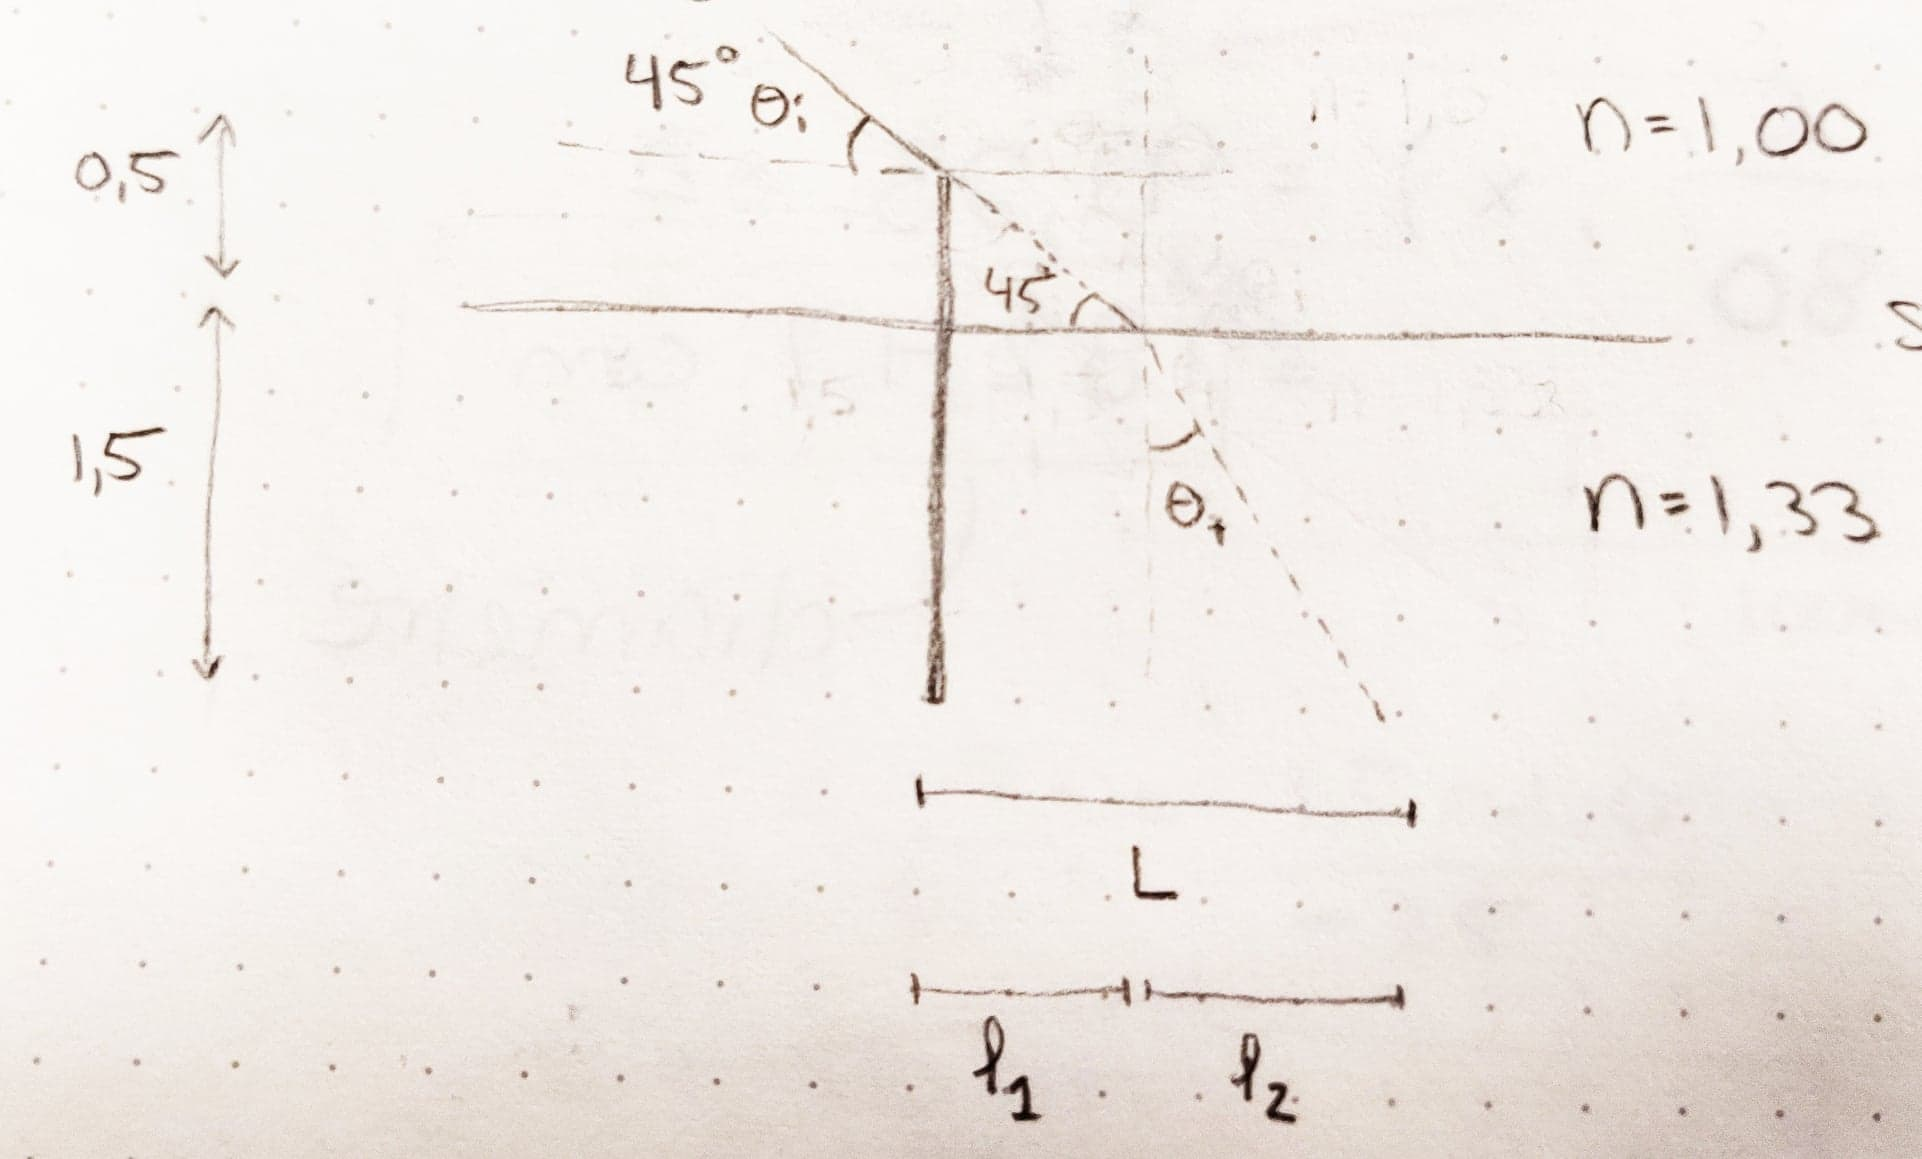
\includegraphics[scale=0.05]{images/graph_ex_refraction.jpg}
        
        \begin{equation*}
        solve = \begin{cases}
            tan(45^\circ) = \frac{0.5}{L_1}\\
            1.00\ sin(45^\circ) = 1.33\ sin(\theta_t) \\
            tan(\theta_t) = \frac{L_2}{1.5}
        \end{cases}
        |\ 0 < \theta_t < 180
        \end{equation*}
        }
        $$\theta_t=32.12^\circ,\ L_1=0.5m,\ L_2=-0.94m$$
        $$|L_1| + |L_2| = 1.44m$$
    \end{minipage}
};
% \node[fancytitle, right=10pt] at (box.north west) {Exercice réfraction};
\end{tikzpicture}

\vfill\columnbreak

% --------------------------------------
\begin{tikzpicture}
\node [mybox] (box){%
    \begin{minipage}{0.3\textwidth}
    $$\frac{n_i}{s_o}+\frac{n_t}{s_i}=\ \frac{n_i}{f_o}=\ \frac{n_t}{f_i}=\ \frac{n_t - n_i}{R}$$

    \txt{
        \textbf{Distance focale objet}\\
        Si $s_i=\infty$ (rayons émergents sont parallèles), alors:
    }
    $$s_o=f_o=\frac{n_i R}{(n_t-n_i)}$$
    
    \txt{
        \textbf{Distance focale image}\\
         Si $s_o=\infty$ (rayons incidents parallèles convergent en un point $f_i$), alors:
    }
    $$s_i=f_i=\frac{n_t R}{(n_t-n_i)}$$
    
    \txt{
        \textbf{Grandissement transversal}\\
        (n = 1 pour une lentille mince ou miroir)
    }
    $$g_t=-\frac{n_i s_i}{n_t s_o} = \frac{h_i}{h_o}$$
    $$g_{total} = g_{t1} \cdot g_{t2} \cdot ... \cdot g_{tn}$$
    
    {\footnotesize
    *Sens des rayons: Objet à l'observateur.\\
    **Si $R\rightarrow\infty$ (ex: ours regarde un saumon directement au dessus de lui), $\frac{n_i}{s_o}+\frac{n_t}{s_i}=0$
    }
    \end{minipage}
};
\node[fancytitle, right=10pt] at (box.north west) {Dioptres sphériques};
\end{tikzpicture}
\begin{tikzpicture}
\node [mybox] (box){%
    \begin{minipage}{0.3\textwidth}
    $\frac{1}{f}=\frac{1}{s_o}+\frac{1}{s_i}=(n_{la}-1)(\frac{1}{R_1}-\frac{1}{R_2})$ où $n_{la}=\frac{n_l}{n_a}$\\
    
    {\footnotesize *Biconvexe: $R_1$ et $-R_2$}
    \end{minipage}
};
\node[fancytitle, right=10pt] at (box.north west) {Lentilles minces};
\end{tikzpicture}
\begin{tikzpicture}
\node [mybox] (box){%
    \begin{minipage}{0.3\textwidth}
    {\footnotesize
    \textbf{Définition:} Lentille considérée comme épaisse lorsque la distance $a$ entre les sommets $V_1$ et $V_2$ des surfaces n'est plus négligeable devant les rayons de courbure des surfaces sphériques. $V_1$ et $V_2$ sont les points gauche et droite de la lentille. $a$ est la distance entre $V_1$ et $V_2$, donc largeur de la lentille.}
    \txt{
        $$\frac{1}{f}\ =\ \frac{1}{s_o}+\frac{0}{s_i}\ =\ (n_{la}-1)[\frac{1}{R_1}-\frac{1}{R_2}+\frac{(n_{la}-1)\ a}{n_{la}\ R_1\ R_2}]$$
        {\footnotesize *où $n_{la}=\frac{n_l}{n_a}$\\}
        
        \textbf{Plans principaux}\\
        {\footnotesize$\bar{V_1 H_1}$ et $\bar{V_2 H_2}$ > 0 lorsque le déplacement de V vers H se fait dans le sens de la propagation de la lumière.}
        $$\bar{V_1 H_1}=\frac{-f(n_{la}-1)\ a}{R_2\ n_{la}}$$
        $$\bar{V_2 H_2} =\ \frac{-f(n_{la}-1)\ a}{R_1\ n_{la}} =\ \bar{V_1 H_1}(\frac{R_2}{R_1})$$
	}
	{\footnotesize
	- $s_o$ et $f_o$ mesurés avec $H_1$, donc $s_o=distance+\bar{V_1H_1}$\\
	- $s_i$ et $f_i$ mesurés avec $H_2$, donc $s_i=s_i+\bar{V_2H_2}$\\ ($solve(\frac{1}{f}=\frac{1}{s_o}+\frac{1}{s_i},s_i)$ puis $s_i=s_i+\bar{V_2 H_2}$)}
    \end{minipage}
};
\node[fancytitle, right=10pt] at (box.north west) {Lentilles épaisses};
\end{tikzpicture}
\begin{tikzpicture}
\node [mybox] (box){%
    \begin{minipage}{0.3\textwidth}
    % \txt{\footnotesize
    %     Il existe une paire de points $f_o$ et $f_i$ ayant les propriétés: 1) Un obj placé en $f_o$ donne des rayons réfléchis parallèles. 2) Des rayons incidents parallèles convergeront en $f_i$
    % }
    $$\frac{1}{f}=\frac{1}{s_o}+\frac{1}{s_i}=\frac{2}{R}$$
    \txt{
    \begin{center}
        \textbf{Si} $s_i=\infty$, \textbf{alors} $s_o=f_o=\frac{R}{2}$,\hskip15pt
        \textbf{Si} $s_o=\infty$, \textbf{alors} $s_i=f_i=\frac{R}{2}$\\
        Donc $f_i=f_o=f=\frac{R}{2}$
    \end{center}
        \textbf{Miroir concave:} Si $R > 0$, alors $f > 0$, 
        \textbf{Miroir convexe:} Si $R < 0$, alors $f < 0$,
        \textbf{Miroir plan:} $R=\infty$ donc $s_i=-s_o$ et $g_t=\frac{-s_i}{s_o}=+1$
    }
    \end{minipage}
};
\node[fancytitle, right=10pt] at (box.north west) {Miroirs};
\end{tikzpicture}

\vfill\columnbreak

% --------------------------------------

\begin{tikzpicture}
\node [mybox] (box){%
    \begin{minipage}{0.3\textwidth}
    \small{
    	\begin{tabular}{>{\raggedleft\arraybackslash}p{4cm}>{\raggedright\arraybackslash}p{3.5cm}}
    	\textit Phase initiale de l'origine ($\varphi$) & 
		    $\omega t_0 + \varphi= tan^{-1}(- \frac{v_0}{\omega x_0})$ \\
		    \noalign{\vskip 2pt}
		    \hdashline[0.5pt/4pt]
		    \noalign{\vskip 2pt}
	    \textit Frequence angulaire ($\omega$) & 
		    $=2 \pi f = \sqrt{\frac{k}{m}} = \sqrt{\frac{g}{l}} $ \\
            \noalign{\vskip 2pt}
		    \hdashline[0.5pt/4pt]
		    \noalign{\vskip 2pt}
	    \textit Periode (T) & 
		    $=\frac{2\pi}{\omega}=\frac{1}{f}$ \\
		    \noalign{\vskip 2pt}
		    \hdashline[0.5pt/4pt]
		    \noalign{\vskip 2pt}
	     \textit Nombre d'onde (k) $m^{-1}$ &
		    $=\frac{\omega}{c}=\frac{2\pi}{\lambda}$ \\
		    \noalign{\vskip 2pt}
		    \hdashline[0.5pt/4pt]
		    \noalign{\vskip 2pt}
	     \textit Longueur d'onde ($\lambda$) &
		    $=c T=\frac{c}{f}$ \\
		    \noalign{\vskip 2pt}
		    \hdashline[0.5pt/4pt]
		    \noalign{\vskip 2pt}
	     \textit Vitesse de l'onde (c) &
		    $=\lambda f = \frac{\omega}{k} = \sqrt{\frac{F}{\mu}}$ \\
		    \noalign{\vskip 2pt}
		    \hdashline[0.5pt/4pt]
		    \noalign{\vskip 2pt}
% 	     \textit Vitesse transversale ($v_y(z,t)$) cm/s &
% 	        $=\frac{\mathrm{d} }{\mathrm{d} t} y(z,t) \newline
% 	        =-A \omega sin(\omega t - k z + \varphi)$
% 		     \\
% 		    \noalign{\vskip 2pt}
% 		    \hdashline[0.5pt/4pt]
% 		    \noalign{\vskip 2pt}
% 	     \textit Acceleration transversale ($a_y(z,t)$) cm/$s^2$ &
% 		    $=\frac{\mathrm{d} }{\mathrm{d} t} v_y(z,t) \newline
% 		    = -A \omega ^2 cos(\omega t - k z + \varphi) \newline
% 		    = - \omega ^2 y(z,t)$ \\
% 		    \noalign{\vskip 2pt}
% 		    \hdashline[0.5pt/4pt]
% 		    \noalign{\vskip 2pt}
% 		 \textit Position max ($x_{max}$) &
% 		    $=A$ \\
% 		    \noalign{\vskip 2pt}
% 		    \hdashline[0.5pt/4pt]
% 		    \noalign{\vskip 2pt}
	     \textit Vitesse max ($v_{max}$) &
		    $=\omega A$ \\
		    \noalign{\vskip 2pt}
		    \hdashline[0.5pt/4pt]
		    \noalign{\vskip 2pt}
	     \textit Acceleration max ($a_{max}$) &
		    $=\omega ^2 A$\\
		    \noalign{\vskip 2pt}
		    \hdashline[0.5pt/4pt]
		    \noalign{\vskip 2pt}
		 \textit Circonférence, Rayon de courbure &
		    $2 \pi r = v_{obj} \cdot T$\\
		    \noalign{\vskip 2pt}
		    \hdashline[0.5pt/4pt]
		    
		    \noalign{\vskip 2pt}
	    \textit Aire d'un cercle &
		    $\pi r^2$\\
		    \noalign{\vskip 2pt}
		    \hline
		    \noalign{\vskip 3pt}
	\end{tabular}}
	
	\begin{tabular}{l|c}
    \begin{minipage}[c]{0.5\textwidth}
        \txt{
        \textbf{\textit{\footnotesize Ondes se propageant en direction de..}} \\
        \textbf{z > 0: }
        $(\omega t - k z)$ et $(k z - \omega t)$ \\
        \textbf{z < 0: }
        $(\omega t + k z)$ et $(- \omega t - k z)$
    }
    \end{minipage} &
    	$v_f=v_i+a\ \Delta t$,\hskip15pt $F=m\cdot a$
    \end{tabular}
    
    \begin{center}
    $sin=\frac{o}{h}$,\quad$cos=\frac{a}{h}$,\quad$tan=\frac{o}{a}$\\
    1 rad = 0.1591549431 circle,\qquad 1 circle = 6.2831853072 rad    
    \end{center}
    
    \end{minipage}
};
\node[fancytitle, right=10pt] at (box.north west) {Révision};
\end{tikzpicture}
\begin{tabular}{lc}
\begin{minipage}[t]{0.15\textwidth}
    \vspace{-2.2cm}
    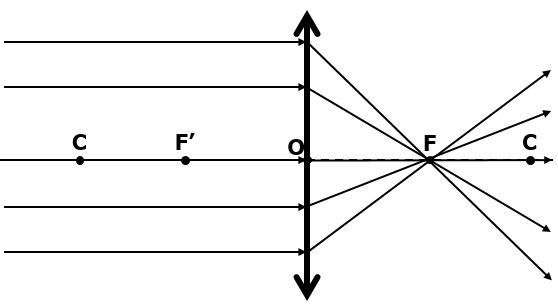
\includegraphics[scale=0.25]{images/lentilles_convergent.jpeg}
\end{minipage} &
    % \vspace{-2cm}
    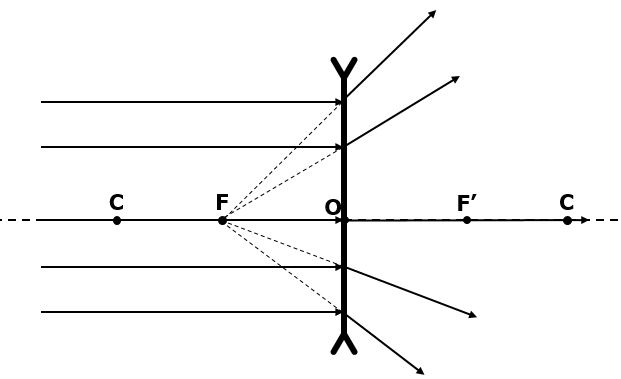
\includegraphics[scale=0.25]{images/lentilles_divergentes.jpeg}
\end{tabular}

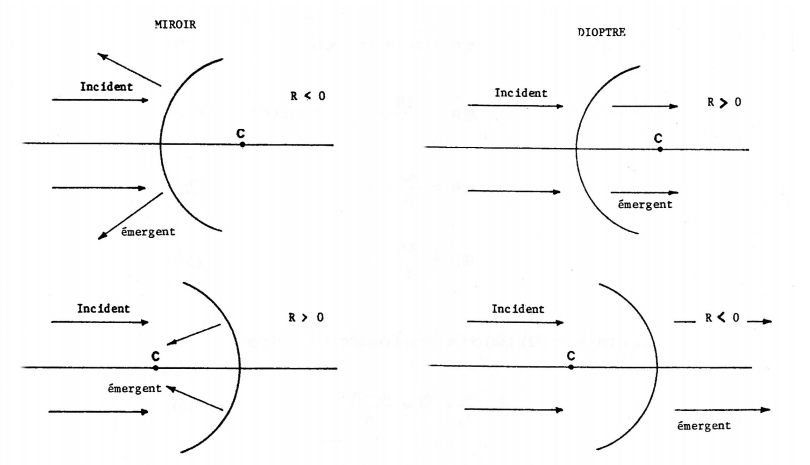
\includegraphics[scale=0.25]{images/miroirs_dioptres.png}

\begin{tabular}{lc}
\begin{minipage}[c]{0.1\textwidth}
    \vspace{-3cm}\hspace{-0.5cm}
    % REQUIRES:
% \usepackage{pgf,tikz,pgfplots}
% \pgfplotsset{compat=1.15}
% \usetikzlibrary{arrows}
\begin{tikzpicture}[line cap=round,line join=round,>=triangle 45,x=1cm,y=1cm, scale=0.55]
\begin{axis}[
    x=1cm,y=1cm,
    axis lines=middle,
    ytick style={draw=none},
    xtick style={draw=none},
    yticklabels={,,},
    xticklabels={,,},
    xmin=-3,
    xmax=3,
    ymin=-3,
    ymax=3]
    \draw [->,line width=1pt] (-2,2) -- (0,0);
    \draw [->,line width=1pt] (0,0) -- (2.4,1.7);
    \draw [->,line width=1pt] (0,0) -- (1.3,-2.2);
    \begin{Large}
        \node [label={[shift={(-0.4,0.5)}]\huge $\theta_i$}] {};
        \node [label={[shift={(0.5,0.5)}]\huge $\theta_r$}] {};
        \node [label={[shift={(0.4,-2)}]\huge $\theta_t$}] {};
        \node [label={[shift={(2.5,0.1)}]\large $n_i$}] {};
        \node [label={[shift={(2.5,-1)}]\large $n_t$}] {};
        \draw[color=black] (1.7,2.1) node {\large Rayon réfléchi};
        \draw[color=black] (-1.8,2.4) node {\large Rayon Incident};
        \draw[color=black] (1.6,-2.5) node {\large Rayon réfracté};
    \end{Large}
\end{axis}
\end{tikzpicture}
\end{minipage} &
    \vspace{-2cm}
    \tdplotsetmaincoords{60}{130}
\begin{tikzpicture}[tdplot_main_coords,line cap=round,>=stealth]
    %B
    \draw[->] (0,0,0) -- (0,0,1.5) node[above=1.05] {\textbf{B} Champ magnétique};
    \draw[color=black] (0,0,2.1) node {\footnotesize (Pouce)};
    
    % E
    \draw[->] (0,0,0) -- (0,2,0) node[below=1.05] {\textbf{E} Champ électrique};
    \draw[color=black] (0,2,-0.6) node {\footnotesize (Majeur)};
    
    % s
    \draw[->] (0,0,0) -- (2,0,0) node[below,pos=1.05] {\textbf{S} Sens de propagation};
    \draw[color=black] (2,0,-0.6) node {\footnotesize (Index)};
    \draw[color=red] plot[variable=\s,domain=0:pi/1.75,samples=100,smooth] ({\s},{0.2*sin(\s*1000)});
    
    % rotation
    \draw [thin, <->, >=stealth'] (0.3,-0.8,0) arc (5:350:5pt and 10pt);
\end{tikzpicture}
\end{tabular}


\vfill\columnbreak

\begin{tikzpicture}
\node [mybox] (box){%
    \begin{minipage}{0.3\textwidth}
    \txt{
        \textbf{\textit{Hauteur d'eau pour voir le fond?}}\\
        $\theta_t=nSolve(tan(\theta_t)=4/2, \theta_t)=63.43^\circ$\\ $\theta_i=nSolve(1.33sin\theta_i=1.00sin(63.43),\theta_i)=42.26^\circ$\\
        $solve(\{tan^{-1}(\frac{4-O}{A})=\theta_i,\ tan^{-1}(\frac{O}{3-A})=\theta_t) \Rightarrow A=1.83=h$
    }
    \end{minipage}
};
% \node[fancytitle, right=10pt] at (box.north west) {Exercice réfraction};
\end{tikzpicture}
\begin{tikzpicture}
\node [mybox] (box){%
    \begin{minipage}{0.3\textwidth}
        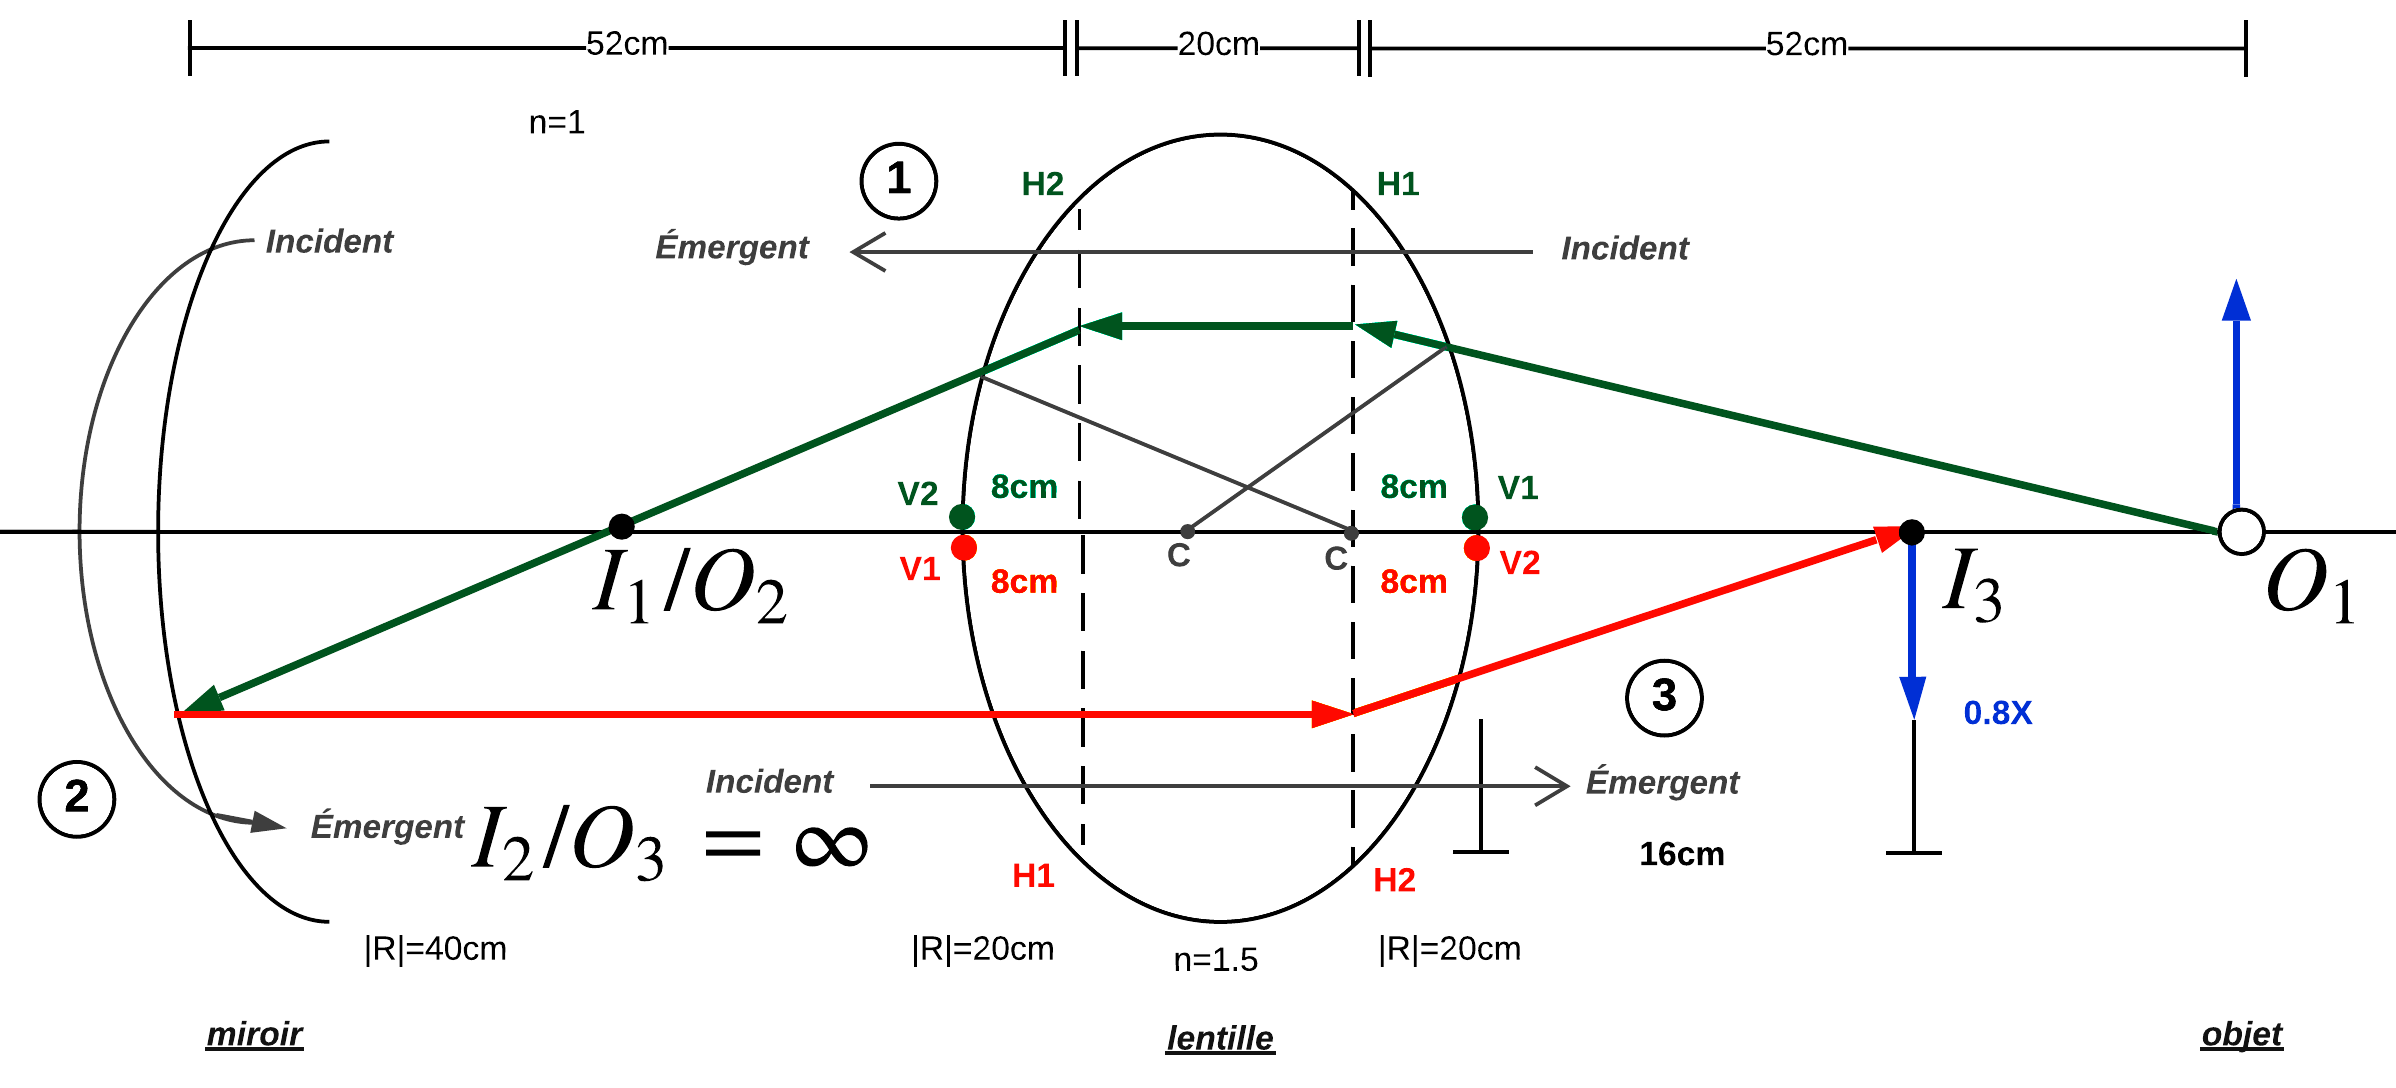
\includegraphics[width=1.04\textwidth]{images/ex_lentille_epaisse.png}
        
        \textbf{Caractéristiques du dioptre}\\
        
        \boxed{$$\frac{1}{f} = (n_{la}-1)[\frac{1}{R_1}-\frac{1}{R_2}+\frac{(n_{la}-1)\ a}{n_{la}\ R_1\ R_2}]$$}
        
        $solve(\frac{1}{f}=(0.5)\cdot (\frac{1}{20}-\frac{1}{-20}+\frac{(n_{la}-1)\cdot20}{n_{la}\cdot20\cdot-20}),f)|n_{la}=\frac{1.5}{1}=+24cm$
        
        \boxed{$$\bar{V_1 H_1}=\frac{-f(n_{la}-1)\ a}{R_2\ n_{la}}$$} $=\frac{-24(n_{la}-1)\ 20}{(-20)\ (n_{la})}=+8cm$\\
        
        \boxed{$$\bar{V_2 H_2} = \bar{V_1 H_1}(\frac{R_2}{R_1})$$} $=(+8)(\frac{-20}{20})=-8cm$\\
        
        \textbf{Interface 1 (lentille)}\\
        
        \boxed{$$s_{o1}=\Delta_{objet,lentille}+\bar{V_1 H_1}$$} $=52cm+(+8)=+60cm$\\
        
        \boxed{$$\frac{1}{f}=\frac{1}{s_o}+\frac{1}{s_i}$$} $=solve(\frac{1}{+24}=\frac{1}{+60}+\frac{1}{s_{i}},s_{i})=40cm$\\
        
        \boxed{$$s_{i1}=s_i+\bar{V_2 H_2}$$} $=40+(-8)=+32cm$\\
        
        $g_t=-\frac{+40}{+60}=-\frac{2}{3}X$\\
        
        \textbf{Interface 2 (miroir)}
        
        \boxed{$$s_{o2}=\Delta_{lentille,miroir}-s_{i1}$$} $=52-32=+20cm$\\
        
        \boxed{$$\frac{1}{s_o}+\frac{1}{s_i}=\frac{2}{R}$$}
        $=solve(\frac{1}{+20}+\frac{1}{s_{i2}}=\frac{2}{R},s_{i2})=false=\infty$
        
        $g_t=-\frac{\infty}{+20}$\\
        
        \textbf{Interface 3 (lentille)}
        
        \boxed{$$s_{o3}=\Delta_{miroir,lentille}-s_{i2}$$} $=\infty$\\
        
        \boxed{$$\frac{1}{f}=\frac{1}{s_o}+\frac{1}{s_i}$$} $=solve(\frac{1}{+24}=\frac{1}{\infty}+\frac{1}{s_i},s_i)=+24cm$\\
        
        \boxed{$$s_{i3}=s_i+\bar{V_2 H_2}$$} $=(+24)+(-8)=16cm$\\
        
        $g_t=-\frac{+24}{\infty}=-24X$
        
        $g_{total}=(-\frac{2}{3})(-\frac{1}{+20})(-\frac{+24}{1})=-0.8X$\\
        
        \textit{\textbf{Réponse:} Image réelle, à 16cm de la droite de la face droite du dioptre.}
    \end{minipage}
};
\node[fancytitle, right=10pt] at (box.north west) {Exercice lentille épaisse};
\end{tikzpicture}


\vfill\columnbreak

\begin{tikzpicture}
\node [mybox] (box){%
    \begin{minipage}{0.3\textwidth}
    \begin{tabular}{>{\raggedleft\arraybackslash}p{3.3cm}>{\raggedright\arraybackslash}p{4.2cm}}
        \tabItem
            {Vitesse de propagation {\scriptsize (OEM)}}
            {$c=\frac{1}{\sqrt{\varepsilon_o\mu_o}}=\frac{E_o}{B_o}$}
    	\tabItem
    	    {Champ électrique\par{\scriptsize($Volt/m$ ou $Watts/Am$)}}
    	    {$E_x(z,t)=E_o sin(\omega t \mp k z + \phi_o)$}
	    \tabItem
    	    {Champ magnétique\par{\scriptsize($Tesla$ ou $Web/m^2$)}}
    	    {$B_y(z,t)=B_o sin(\omega t \mp k z + \phi_o)$}
	    \tabItem
    	    {Intensité de l'OEM\par{\scriptsize(Vecteur de Poynting). S est parallèle à la propagation. ($Watts/m^2$)\par **$E_o$ et $B_o$ sont l'AMPLITUDE}}
    	    {
        	    $\vec{S}=\frac{\vec{E}\times\vec{B}}{\mu_o}$\par
        	    $I_{moy}=\frac{E_o\ B_o}{2\ \mu_o}=\frac{c_o\ B_o^2}{2\ \mu_o}=\frac{E_o^2}{2\ \mu_o c_o}$
    	    }
	    \tabItem
    	    {Loi de Wien\par{\scriptsize (située dans l'infrarouge) ($m\cdot ^\circ K$)}}
    	    {$\lambda_{max}T= 2.898\times10^{-3}$}
	    \tabItem
    	    {Loi de Stefan-Boltzmann {\scriptsize ($I=\frac{Watts}{m^2}$), ($L=Watts$)}}
    	    {
        	    $I=\sigma(T^4-T_o^4)$\par
        	    $L=I\cdot Aire$, {\scriptsize $\sigma$= cte. de Boltzmann\par
    	    $T=temperature + Kelvin$}
    	    }
	    \tabItem
    	    {Qte de mouvement du photon {\footnotesize ($Kg\frac{m}{s}$)}}
    	    {$p=\frac{E}{c} = \frac{hf}{c}$\par{\scriptsize     	    tel que $E=mc^2$ ET $m=\frac{E}{c^2}$, \hskip3pt
    	    $p=mv$ ET $m=\frac{p}{c}$}}
	    \tabItem
    	    {" sur une surface absorbante}
    	    {$p= m_B v_B =\frac{U}{c}$}
	    \tabItem
    	    {" sur une surface réfléchissante}{$p=m_B v_B =\frac{2U}{c}$}
	    \tabItem
    	    {" sur une surface partiellement réfléchissante}
    	    {$p=m_B v_B=(R+1)\frac{U}{c}$\par{\scriptsize (si une fraction R $(0<R<1)$ des photons est réfléchie par la surface)}}
	    \tabItem
	        {Pression de radiation {\scriptsize($\frac{N}{m^2}$)}}
	        {$P=\frac{F}{A_\bot}=\frac{(R+1)}{c}I$,  {\scriptsize où $I=S_{moy}$}}
        \tabItem
            {Distance entre S et O}
            {$solve(d=c \Delta t,\ d)$\par{\scriptsize (2d si allé-retour)}}
        \tabItem
            {Amplitude}
            {$A=\sqrt{E_x^2+E_y^2+E_z^2}=E_o\ V/m$}
	\end{tabular}
	{\footnotesize
	\textcolor{blue}{$A_\bot$}: Aire de la surface éclairée par la lumière.
	\textcolor{blue}{$F$}: Force exercée sur la surface éclairée par la lumière.
	\textbf{Pression de radiation:} Si on place un obstacle sur le parcourt d’un rayonnement électromagnétique, celui-ci ressentira une \textit{force résultante} qui tentera de le \textit{déplacer} dans le sens de la propagation.
	}
    \end{minipage}
};
\node[fancytitle, right=10pt] at (box.north west) {Optique physique};
\end{tikzpicture}
\begin{tikzpicture}
\node [mybox] (box){%
    \begin{minipage}{0.3\textwidth}
    \txt{\footnotesize
        \begin{minipage}{0.5\textwidth}
            \textbf{Effet Doppler} variation de fréquence en cas de mouvement relatif entre la source et l'observateur.\\
            
            \textbf{Vitesse} relative de la source par rapport à l'observateur: $\vec{v}=\vec{v_s}-\vec{v_o}$
            
            $$f_o=f_s(\frac{\sqrt{1-(\frac{v}{c})^2}}{1+\frac{v}{c}cos(\theta)})^N$$
            {\footnotesize *N est le nombre d'allé-retour.}\\
            
        	\textbf{Effet transversale:} Si $\theta=90^\circ$ alors $f_o<f_s$\\
        	
        	\textbf{Déplacement Doppler}
            $$\Delta\lambda=\lambda_o - \lambda_s$$
            $$\lambda_o=\lambda_s (\frac{1+\frac{v}{c}cos(\theta)}{\sqrt{1-(\frac{v}{c})^2}})$$
            $$\frac{\Delta \lambda}{\lambda_s}=(\frac{1+\frac{v}{c}cos(\theta)}{\sqrt{1-(\frac{v}{c})^2}}-1)$$
            \textbf{Cas particulier}\\
            Si $\frac{v}{c}<<1$ ou $\frac{\Delta\lambda}{\lambda}<<1$ alors:\\
            $\frac{\Delta \lambda}{\lambda_s}=\frac{v}{c}cos(\theta)$
        \end{minipage}
        \begin{minipage}{0.35\textwidth}
            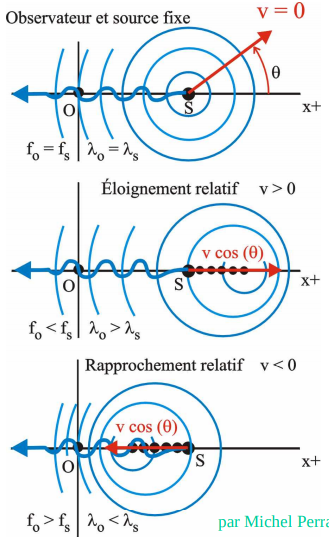
\includegraphics[scale=0.34]{images/effet_doppler.png}
        \end{minipage}
    }
    \end{minipage}
};
\node[fancytitle, right=10pt] at (box.north west) {Doppler};
\end{tikzpicture}

\vfill\columnbreak

\begin{tikzpicture}
\node [mybox] (box){%
    \begin{minipage}{0.3\textwidth}
    \begin{tabular}{p{0.3\textwidth} p{0.61\textwidth}}
      \vspace{-5pt}\hspace{-0.8cm} 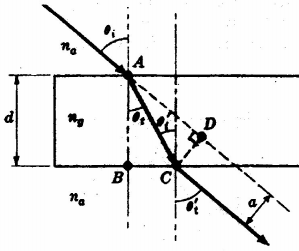
\includegraphics[scale=0.3]{images/ex_8.png} &
      \vspace{-8pt}
      \txt{
        \hspace{-0.5cm}
        \textbf{\textit{a) Angle du rayon lumineux sortant de la plaque?}}
        \par\hspace{-0.5cm}
        Interface 1:
        \par\hspace{-0.5cm}
        $nSolve(1.0sin30^\circ = 1.5sin\theta_{t1}, \theta_{t1})=19.47^\circ$
        \par\hspace{-0.5cm}
        Interface 2:
        \par\hspace{-0.5cm}
        $nSolve(1.5sin\theta_{t1} = 1.0sin\theta_{t2}, \theta_{t2})=30^\circ$
        \par\hspace{-0.5cm}
        $\alpha = 30 - 19.47$
        \par\hspace{-0.5cm}
        \textbf{\textit{b) Déplacement latéral "a" du rayon lumineux?}}
        \par\hspace{-0.5cm}
        $b\cdot cos \theta_{t1} \Rightarrow b=5.3cm$
        \par\hspace{-0.5cm}
        $5.3 sin (\theta_{t2}-\theta_{t1})=a=0.97cm$
      }
    \end{tabular}
    \end{minipage}
};
% \node[fancytitle, right=10pt] at (box.north west) {Exercice optique physique};
\end{tikzpicture}
\begin{tikzpicture}
\node [mybox] (box){%
    \begin{minipage}{0.3\textwidth}
    \newcommand{\warning}[1]{\textcolor{red}{\footnotesize\textit{#1}}}
    \begin{tabular}{p{0.3\textwidth} p{0.61\textwidth}}
      \vspace{-10pt}\hspace{-0.85cm} 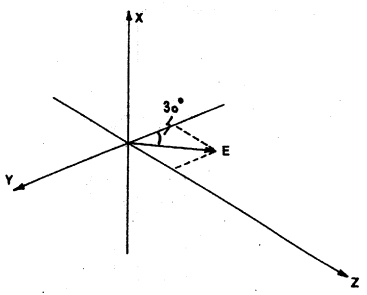
\includegraphics[scale=0.25]{images/ex_optique_physique.png} &
      \vspace{-8pt} {
          \txt{\textit{
          Un laser émet un faisceau lumineux de rayon $r_L=1cm$ selon l'axe X négatif. Fréquence $f=10^{12}Hz$. Champ électrique possède une amplitude $E_o=10^5 V/m$. \textbf{a)} Expression de l'OEM E et B?
          \textbf{b)} Laser frappe en son centre une plaque métallique avec un coeff. de réflexion $R=0.4$; $m=0.5$ grammes; diamètre $d_p=1cm$. Temps écoulé en heures si un observateur situé sur la plaque métallique mesure un $\lambda_o$ qui diffère de 0.8nm de celle émise par le laser $\lambda_s$? Hypothèse: $v<<c$.}
          }
      }
    \end{tabular}
    \txt{
        \def \w {2\cdot 10^{12}\pi}
        \def \k {2.1\cdot10^4}
        
        \textbf{a)} $f=10^{12}Hz$, $E_o=10^5V/m$\\
        $\rightarrow$ $\boxed{\omega=2\pi f}=2\cdot \pi \cdot 10^{12}=2\times 10^{12}\pi$ rad/s\\
        $\rightarrow$ $\boxed{k=\omega/c}=\omega\cdot3\times 10^8=2.095\times10^4$ rad/m\\
        $\Vec{S}$ se propage vers z < 0 donc $E=E_ocos(\omega t - k z)$ (angle \textit{cos} rapport à z)\\
        \textbf{Pour le champ électrique $E$:}\\
        $\rightarrow$ $E_x=0$ V/m \textbf{et} $E_y=(-)E_o\cdot cos 30^\circ$\warning{*} V/m \textbf{et} $E_z=E_o cos 60^\circ$ V/m\\
        \dbox{$E(z,t)=[0\ _i E_y\ _j + E_z\ _k] cos (\w t + \k z)\ V/m$}\warning{**}
        
        \warning{*TOUJOURS REGARDER la direction sur l'axe pour les signes négatif}\\
        \warning{**Angle du vecteur E cos par rapport à Z}
        
        \textbf{Pour le champ magnétique $B$:}
        $\boxed{c=\frac{E_o}{B_o}}\Rightarrow B_o=3.3\cdot 10^{-4}$ Tesla\\
        $\rightarrow$ $B_x=0$ V/m \textbf{et} $B_y=B_o\cdot sin 30^\circ$ V/m \textbf{et} $B_z=B_o cos 30^\circ$ V/m\\
        $\rightarrow$ \dbox{$B(z,t)=[0\ _i B_y\ _j + B_z\ _k] cos (\w t + \k z)\ V/m$} T \warning{*}\\
        \warning{*Angle du vecteur B cos par rapport à Z}
        
        \textbf{b)} $R=0.4$, $m=0.5g$, $r_L=1cm$, $d_p=1cm$, $\Delta\lambda=0.8nm$\\
        \textbf{Selon x:} $\boxed{\vec{v}=\vec{v_s}-\vec{v_o}}=0-(-\vec{v_o})=\vec{v_o}$\\
        $\vec{v}>0 \Rightarrow$ donc éloignement relatif et $f_o<f_s$\\
        \warning{*Faire graphique AVEC la direction du x. Laser fait de la pression de radiation sur la plaque (obs) qui se déplace et le laser (src) est immobile par rapport à l'obs.}\\
        $\rightarrow$ $\boxed{c=\lambda_s/f_s}\Rightarrow\ 3\cdot  10^8=\lambda_s\cdot 10^12\Rightarrow \lambda_s=3\cdot 10^{-4}$\\
        $v<<c$ donc $v/c<<1$ alors $\boxed{\Delta \lambda/\lambda_s=1+\frac{v}{c}cos\theta-1}$\\
        $\rightarrow$ $solve(\frac{0.8\cdot 10^{-9}}{3\cdot 10^{-4}}=1+\frac{v}{3\cdot 10^8} cos 0^\circ, v) \Rightarrow$ \dbox{$v_o=800.25$ m/s}\\
        $\rightarrow$ $\boxed{P=\frac{(R+1)}{c}I=\frac{F}{A_\bot}} \Rightarrow \boxed{F=ma}=0.0005kg\cdot a$\\
        $\Rightarrow \boxed{I=\frac{E_o\ B_o}{2\_\mu_o}}=1.33\cdot 10^{-7} \Rightarrow \boxed{A_\bot} = \pi (d_p/2)^2=0.79cm^2$\\
        $\Rightarrow solve(\frac{(R+1)}{\_c}I=\frac{m\cdot a}{A_\bot \_cm}, a) \Rightarrow a=0.0097 m/s^2$ \warning{*Attention cm vs. m}\\
        $\boxed{v_f=v_i+a\Delta t}=800=0+0.001 \cdot \Delta t \Rightarrow \Delta t = 800000s = 222 heures$
        
    }
    \end{minipage}
};
\node[fancytitle, right=10pt] at (box.north west) {Exercice optique physique};
\end{tikzpicture}

\end{multicols*}
\end{document}